\documentclass[11pt]{IEEEtran}
\IEEEoverridecommandlockouts
% The preceding line is only needed to identify funding in the first footnote. If that is unneeded, please comment it out.
\usepackage{cite}
\usepackage{amsmath,amssymb,amsfonts}
\usepackage{algorithmic}
\usepackage{hyperref}
\usepackage{graphicx}
\usepackage{textcomp}
\usepackage{float}
\usepackage{xcolor}
\usepackage{circuitikz}
\usepackage[english]{babel}
\usepackage{titlesec}
\usepackage{caption}
\usepackage{svg}
\captionsetup{belowskip=-10pt}  % Reduce space below captions
\def\BibTeX{{\rm B\kern-.05em{\sc i\kern-.025em b}\kern-.08em
    T\kern-.1667em\lower.7ex\hbox{E}\kern-.125emX}}


\title{Detection and Classification of Short Circuits in Power System Transmission Lines using RNN\\
}


\author{\IEEEauthorblockN{Harun Špago} \\
\IEEEauthorblockA{\textit{University of Sarajevo}} \\
\IEEEauthorblockA{\textit{Faculty of Electrical Engineering Sarajevo}} \\
\IEEEauthorblockA{\textit{Department of Automation and Electronics} \\
\textit{B\&H, Sarajevo}\\
Emails: hspago1@etf.unsa.ba}\\
}

\begin{document}

\maketitle

\begin{abstract}
This paper addresses the problem of detecting and classifying short circuits in power system transmission lines using deep learning methods. A neural network based on GRU (\textit{Gated Recurrent Unit}) and LSTM (\textit{Long Short-Term Memory}) architectures was implemented to improve the accuracy and speed of fault detection. The input data consisted of voltages and currents in a three-phase system, while the network outputs represented seven different types of faults.

The model was trained using ten epochs and a GPU, with different window sizes applied. 

The implemented model enables \textit{real-time} fault detection, contributing to the reliability and security of power systems. These results demonstrate that neural networks can significantly enhance the efficiency and speed of fault identification compared to traditional protection methods.
\end{abstract}

\begin{IEEEkeywords}
short circuit, power system, neural networks, GRU, LSTM, sliding window, fault classification, \textit{real-time} detection
\end{IEEEkeywords}

\section{Introduction}
In the era of Industry 4.0, the demand for electrical energy is constantly increasing, leading to a rise in the number of production units connected through a complex power system (PS). This system consists of three main components: generation, transmission, and distribution. The stable and reliable operation of the PS is crucial to minimizing impacts on industry, transportation, and households. 
However, system faults can cause major supply interruptions and significant financial losses, making fast fault detection and isolation essential.\\
Short circuits are one of the most common causes of power outages, occurring due to weather conditions, equipment failures, human factors, or contact with animals. These faults destabilize the system and lead to large energy losses. Traditionally, system protection is carried out using relays and circuit breakers, but their response time can be slow.
Various algorithms have been introduced. Paper \cite{8442440} presents a wavelet-based short-circuit identification algorithm (using MATLAB’s \textit{symlet4}) for double-sided power lines, validated through simulations and a real-world five-node closed-loop lab system.
Paper \cite{7806061} presents a more natural way of looking at this problem. They proposes a novel short-circuit fault detection method using instantaneous voltage measurements and derivatives, deriving an exact analytical solution from telegraph equations for signal propagation


Nowadays machine learning and deep learning methods are being used for faster and more accurate fault detection and classification. As shown in \cite{9787450} numerous different algorithms can be used to detect faults, and more like control algoithms etc.
Machine learning has emerged as a powerful and nowadays popular tool for automatically extracting complex patterns from data, offering the potential to significantly enhance the accuracy and efficiency of fault detection in transmission lines. In recent years, there has been a notable surge in research focused on leveraging machine learning algorithms to address challenges in this domain. 
As shown in \cite{10709384} ML can have a significant role in optimizing smart grids across six key areas—demand forecasting, fault detection, and renewable integration—while addressing challenges like scalability and data privacy to enhance grid reliability and future innovation.
Study presented in \cite{10435012} demonstrates that Sequential Neural Networks (SNN) achieve superior performance over K-Nearest Neighbors (KNN) for fault detection in power transmission lines.
Another advantage of using MLs is historicly available data for a certain unit, in paper \cite{10129641} ML and deep learning models are used to predict fault-prone Remote Terminal Units (RTUs) by leveraging historical activity data, optimizing maintenance prioritization through rigorous experimental design, feature engineering, and model evaluation.
Various neural network algorithms, such as recurrent neural networks (RNNs)\cite{9498552}, convolutional neural networks (CNNs), and artificial neural networks (ANNs). In \cite{9493498} ANNs are used for detecting faults in Insulated Gate Bipolar Transistor (IGBT). 
In paper \cite{10409468} methods like PCA (Pricipal Component Analysis) along with classification method like SVN (Support Vector Machine) are used to detect short circuits in transformator windings.
Simple ML methods such as Decision Threes (DTs) can be used for short circuit detection as well \cite{9264078}.
Although effective, many of these methods are computationally demanding and complex to implement. 


This paper explores short circuit detection and classification in PS with the aim of improving detection speed and accuracy, the goal is to produce a real-time predictor that is able to receive needed inputs for classification in this case the system variables that are needed are three phase voltages and three line currents. The analysis is going to be based around recurrent neural networks (RNNs). 
We decided to analyise the behaviour of LST (Long Short-Term Memory) networks and GRU (Gated Reccurent Unit) networks. Also this paper introduces a slidig window. Simple said that the input of the neural network will not be a vector only containing the current voltage and current values, it is also going to need $WINDOW\_SIZE - 1$ past inputs i order to get a better and more precise prediction. This window will slide as new samples come in so that in each moment we have the current sample and $WINDOW\_SIZE - 1$ past samples. 
At the end of the paper we will present the value of the detection delay. This is the time that passes from the moment the fault occurs to the moment the neural network signal the fault. The goal is to have this time as much smaller as possible, but this time is also very dependent on the sampling rate of the system itself.

\subsection{Dataset}
For training the neural network, an appropriate dataset needs to be generated. The input to the neural network will consist of phase voltages and line currents, namely voltages \textit{$V_a$, $V_b$} and \textit{$V_c$} and currents \textit{$I_a$, $I_b$} and \textit{$I_c$}. The data will be generated based on the mathematical model of the transmission line where the fault occurred. Figure \ref{fig:transmission_line} shows the transmission line model under consideration.

\begin{figure*}[t]  % Note the asterisk (*) for two-column figures
    \centering
    \includesvg[width=\textwidth]{figs/drawing.svg}  % Use full \textwidth
    \caption{Transmission line model}
    \label{fig:transmission_line}  % Fixed label (avoid numbers)
\end{figure*}

Unknown parameters in the figure are:
   \begin{itemize}
    \item \( V_{abc} \) - phase voltages, one of the network inputs,
    \item \( I_{abc} \) - line currents, one of the network inputs,
    \item \( I_{abc}^f \) - fault current,
    \item \( I_{abc}^p \) - load current,
    \item \( R \) - line resistance,
    \item \( L \) - line inductance,
    \item \( C \) - shunt capacitance,
    \item \( R_f \) - fault resistance.
   \end{itemize}
Using \textit{Kirchhoff's} laws, a state-space representation of the system can be obtained, which will be used for data generation.

Applying \textit{Kirchhoff's} current law, the following equations are obtained:
\begin{equation}
    I_{abc} = I_{abc}^{1} + I_{abc}^{2} + I_{abc}^{f}
\end{equation}

\begin{equation}
    I_{abc}^{1} = I_{abc}^{3} + I_{abc}^{p} 
\end{equation}

Equations derived using \textit{Kirchhoff's} voltage law are:

\begin{equation}
    I_{abc}^{2} = C \cdot \frac{dV_{abc}}{dt} 
\end{equation}

\begin{equation}
    I_{abc}^{f} = \frac{V_{abc}}{R_f}
\end{equation}

\begin{equation}
    V_{abc} = R \cdot I_{abc}^{1} + L \cdot \frac{d I_{abc}^{1}}{dt} + \frac{1}{C} \cdot \int_{ \infty}^{t} I_{abc}^{3} \, dt
\end{equation}
Substituting equation (2) into (5) yields:
\begin{equation}
    V_{abc} = R \cdot I_{abc}^{1} + L \cdot \frac{d I_{abc}^{1}}{dt} + \frac{1}{C} \cdot \int_{ \infty}^{t} (I_{abc}^{1} - I_{abc}^{p})  \, dt
\end{equation}

Differentiating the previous equation, we obtain:
\begin{equation}
   \frac{d V_{abc}}{dt} = R \cdot  \frac{d I_{abc}^{1}}{dt} + L \cdot \frac{d^2 I_{abc}^{1}}{dt^2} + \frac{1}{C} \cdot I_{abc}^{1} - \frac{1}{C} \cdot I_{abc}^{p}
\end{equation}


\section{Used Algorithm}
For the purpose of detecting and classifying short circuits in the power system, a recurrent neural network was used, which will be discussed in more detail below. The data is organized into two CSV files:
\begin{itemize}
    \item inputs.csv - contains 6 input features (three phase voltages and three line currents),   
    \item outputs.csv - contains 1 output value representing the type of detected short circuit. 
\end{itemize}
The goal is to train the model so that it can analyze data in real-time and classify fault types.
If the neural network is to be suitable for \textit{real-time} application, instead of processing all data at once, a sliding window approach is used. This means that at any given moment, the model uses the current input sample and the previous $N$ samples, allowing for the analysis of the temporal dynamics of the signal. The size of $N$ can be adjusted to optimize model accuracy.

\subsection{Signal Preprocessing}
Before the data is used for training the neural network, proper preprocessing must be performed to ensure model efficiency and improve classification accuracy. The main goal of preprocessing is to adapt the data to be suitable for the neural network, reduce noise effects, and enable faster model convergence. 

One of the key steps in preprocessing is normalizing the input data. Voltage and current values are divided by the nominal voltage and current values of the system, i.e., the transmission line, to ensure a uniform data scale. This achieves:
\begin{itemize}
    \item preventing the dominance of certain variables due to their large absolute values,
    \item improving the stability of neural network training,
    \item enabling faster and more efficient model convergence,
    \item reducing the network's sensitivity to extreme values.
\end{itemize}

This normalization is especially important because neural networks perform better when input data is within a specific numerical range. Additionally, in real systems, different sensors may have different measurement ranges, so it is crucial to bring all values to the same scale.

\subsection{Data Processing}

For the neural network to learn effectively and make accurate decisions, the data must go through several processing steps. These steps ensure that the network receives high-quality and consistent input data, which directly impacts model accuracy.

The first step in data processing is loading it from CSV files containing information about voltages, currents, and fault types. The input data comes from the file \textit{inputs.csv} and consists of six numerical features (three phase voltages and three line currents), while the file \textit{outputs.csv} contains integer labels representing the type of short circuit.\\

%\subsubsection*{Short Circuit Classification}

The output of the neural network represents a multi-class classification problem, where the model must recognize and classify a given signal into one of eight classes. Each class corresponds to a specific system state:

\begin{itemize}
    \item \textbf{class 0} – normal system state (no fault),
    \item \textbf{class 1} – short circuit of phase L1 to ground,
    \item \textbf{class 2} – short circuit of phase L2 to ground,
    \item \textbf{class 3} – short circuit between phases L1 and L2,
    \item \textbf{class 4} – short circuit of phase L3 to ground,
    \item \textbf{class 5} – short circuit between phases L1 and L3,
    \item \textbf{class 6} – short circuit between phases L2 and L3,
    \item \textbf{class 7} – three-phase short circuit (L1, L2, and L3).
\end{itemize}

To avoid errors during model training, it is necessary to check the data for missing values. If there are missing values, they can be removed or interpolated to ensure data continuity. The most commonly used methods are deleting rows with missing values or filling them using the mean, median, or linear interpolation.

Since the model is designed for \textit{real-time} data processing, the sliding window method is used. Instead of analyzing each sample separately, the neural network uses a set of \(N+1\) consecutive samples to recognize temporal patterns in the data. Thus, the input to the model has the shape:
\vskip -10pt
\begin{equation}
(N+1, 6)
\end{equation}
where $N$ represents the number of previous samples used for prediction. This method allows the network to utilize the temporal dependence between data points, thereby increasing the accuracy of fault classification.

To ensure good model generalization, the data is divided into training and test sets. It is essential that the data remains temporally consistent to prevent information leakage between sets. A typical data split is:
\begin{itemize}
    \item training set – 80\% of the data, used for model training,
    \item test set – 20\% of the data, used for model evaluation.
\end{itemize}

During data splitting, a sequential sampling principle is used, where test data is taken from the last portion of the dataset to ensure the model is tested on data it has not seen during training.

\subsection{Neural Network Architecture}

Due to the temporal nature of the data, several approaches were considered when designing the neural network architecture:

\begin{itemize}
    \item recurrent neural network (RNN) – using LSTM or GRU layers to analyze sequential data, allowing the network to recognize temporal dependencies between input samples, which is crucial for detecting faults with a dynamic nature
    
    \item convolutional neural network (CNN 1D) – uses convolutional filters to analyze local temporal patterns in the data, which can help identify sudden changes in voltages and currents that signal faults
    
    \item \textit{feed-forward} neural network (DNN) – the simplest model that uses fully connected layers, does not capture temporal relationships between consecutive measurements, making it less suitable for this problem.
\end{itemize}

In this work, GRU (\textit{Gated Recurrent Unit}) and LSTM (\textit{Long Short-Term Memory}) networks, which are types of recurrent neural networks, were used for the analysis of time series and sequential data. LSTM networks have additional memory cells that better retain long-term dependencies in data, while GRU uses a simpler approach with fewer parameters, making it faster and more efficient for training. In this case, the combination of LSTM and GRU allows the model to better detect patterns in voltage and current signals, improving the accuracy of short-circuit classification in the power system.

%For performance optimization, the network was configured with:

%\begin{itemize}
 %   \item \textbf{Adam optimizer} for fast convergence and efficient weight adaptation.
 %    \item \textbf{Sparse categorical crossentropy} as the loss function since the output values are discrete (fault classification).
 %   \item \textbf{Accuracy metric tracking} to measure the model’s efficiency.
%\end{itemize}

\subsection{Model Training and Testing}

Training and evaluating the model are key steps in ensuring accurate short-circuit classification. The steps include:

\begin{enumerate}
    \item model training – \textit{batch} data generation was performed to optimize memory consumption when processing large datasets; data was split into training (80\%) and test (20\%) sets

    \item \textit{real-time} inference – after training, the model maintains a \textit{buffer of the last \(N\) samples}, where each new sample is added to the buffer, and the oldest one is removed
    
    \item validation and testing – the model was tested on real and simulated data to ensure its robustness (test results were saved in the files \textit{predicted\_predictions\_gru\_model\_window\_15.npy} and \textit{true\_predictions\_gru\_model\_window\_15.npy})
\end{enumerate}
A script, \textit{plot\_data.py}, was created for result visualization, allowing the display of model predictions compared to actual values from the \textit{dataset}.

\subsection{Model Training Results}

For model training, \textbf{10 epochs} and a graphics processing unit (GPU) were used to accelerate the processing of large amounts of data. LSTM and GRU neural networks were tested with different window sizes (WINDOW\_SIZE) to analyze their performance and accuracy in fault classification. Specifically, window sizes of \textbf{5, 10, and 15} were tested. The models were saved in \textit{.h5} format for later evaluation, and the best results were achieved with a window size of \textbf{15}, while smaller windows (e.g., size 5) resulted in lower accuracy due to insufficient data for analysis.


\section{Simulation Results}
In this section, the simulation results for detecting and classifying short circuits in the power system using the GRU neural network are analyzed. The graphical representations indicate the actual and predicted outputs of the model, along with potential prediction errors.
The simulation results are as follows:

\begin{enumerate}

    \item LSTM networks:
    \begin{itemize}
        \item WINDOW\_SIZE = 10: where an accuracy of \textbf{99.20\%} was achieved.
        \item WINDOW\_SIZE = 15: The model was trained on the same number of samples but with a larger time window, achieving an even better accuracy of \textbf{99.85\%}.
    \end{itemize}
    
    \item GRU networks:
    \begin{itemize}
        \item WINDOW\_SIZE = 15 with 16 units in the hidden layer: \textbf{99.16\%}.
        \item WINDOW\_SIZE = 15 with 8 units: \textbf{97.46\%} accuracy.
        \item WINDOW\_SIZE = 15 with 2 units: \textbf{95.46\%} accuracy.
    \end{itemize}
\end{enumerate}

The analysis shows that increasing the time window size (\textbf{W}INDOW\_SIZE) contributes to improving accuracy but also increases model complexity and training time. Additionally, a higher number of units in the hidden layer of the GRU network results in better performance, but overly complex models can lead to overfitting. LSTM proved to be more accurate for this type of problem, especially when using a larger time window.

These findings confirm that a combination of LSTM and GRU networks, along with optimization of WINDOW\_SIZE and the number of units, can achieve high accuracy in real-time classification of short circuits in the power system.

The displayed graph (Figure \ref{2}) shows the prediction of the GRU model with 8 neurons and a window size of 15. The blue line represents actual outputs, while the red dashed line indicates model predictions. It is evident that the model struggles with prediction stability at the beginning of the sequence but aligns with real data in the later part. Errors are present during transitions between different fault classes.

\begin{figure}[H]
    \centering
    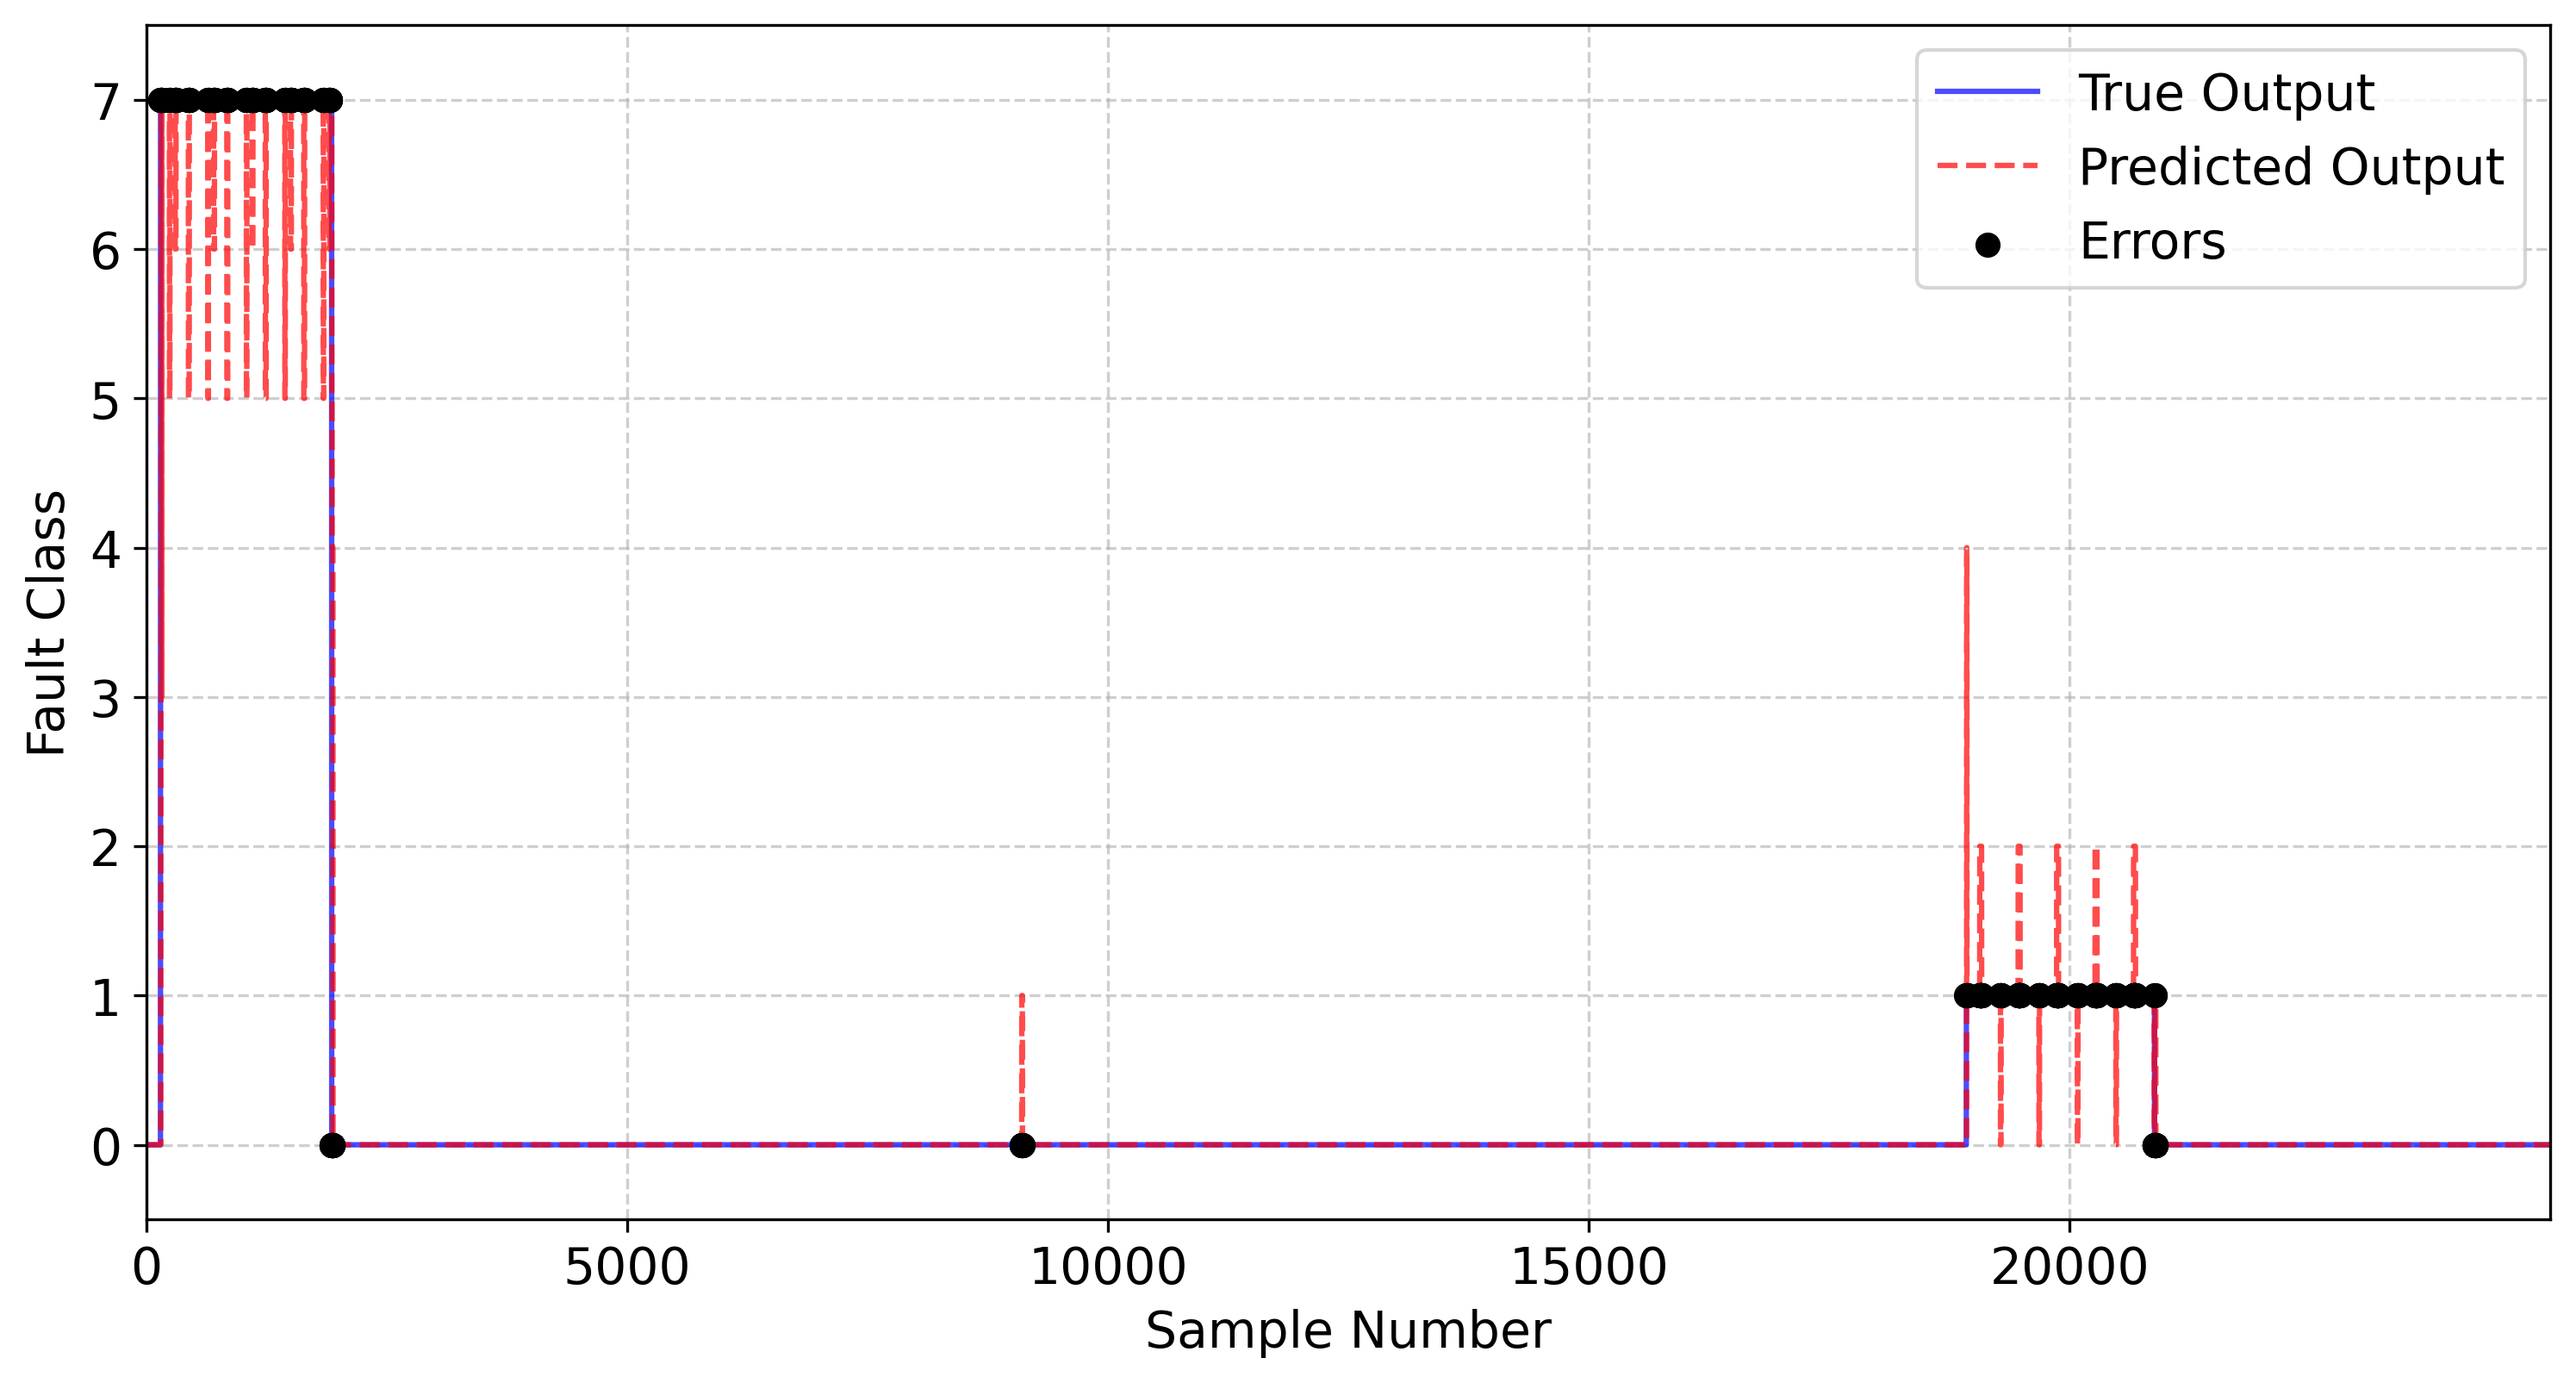
\includegraphics[width=1\linewidth]{figs/true_vs_predicted_gru_minimum_model_window_size_15.png}
    \caption{GRU model with 8 neurons and a window size of 15}
    \label{2}
\end{figure}
The following figure \ref{fig:ekstra_minimum} analyzes the GRU model with 2 neurons and a window size of 15. The model shows poorer stability compared to the previous one, with visible large fluctuations in detected faults.

\begin{figure}[H]
    \centering
    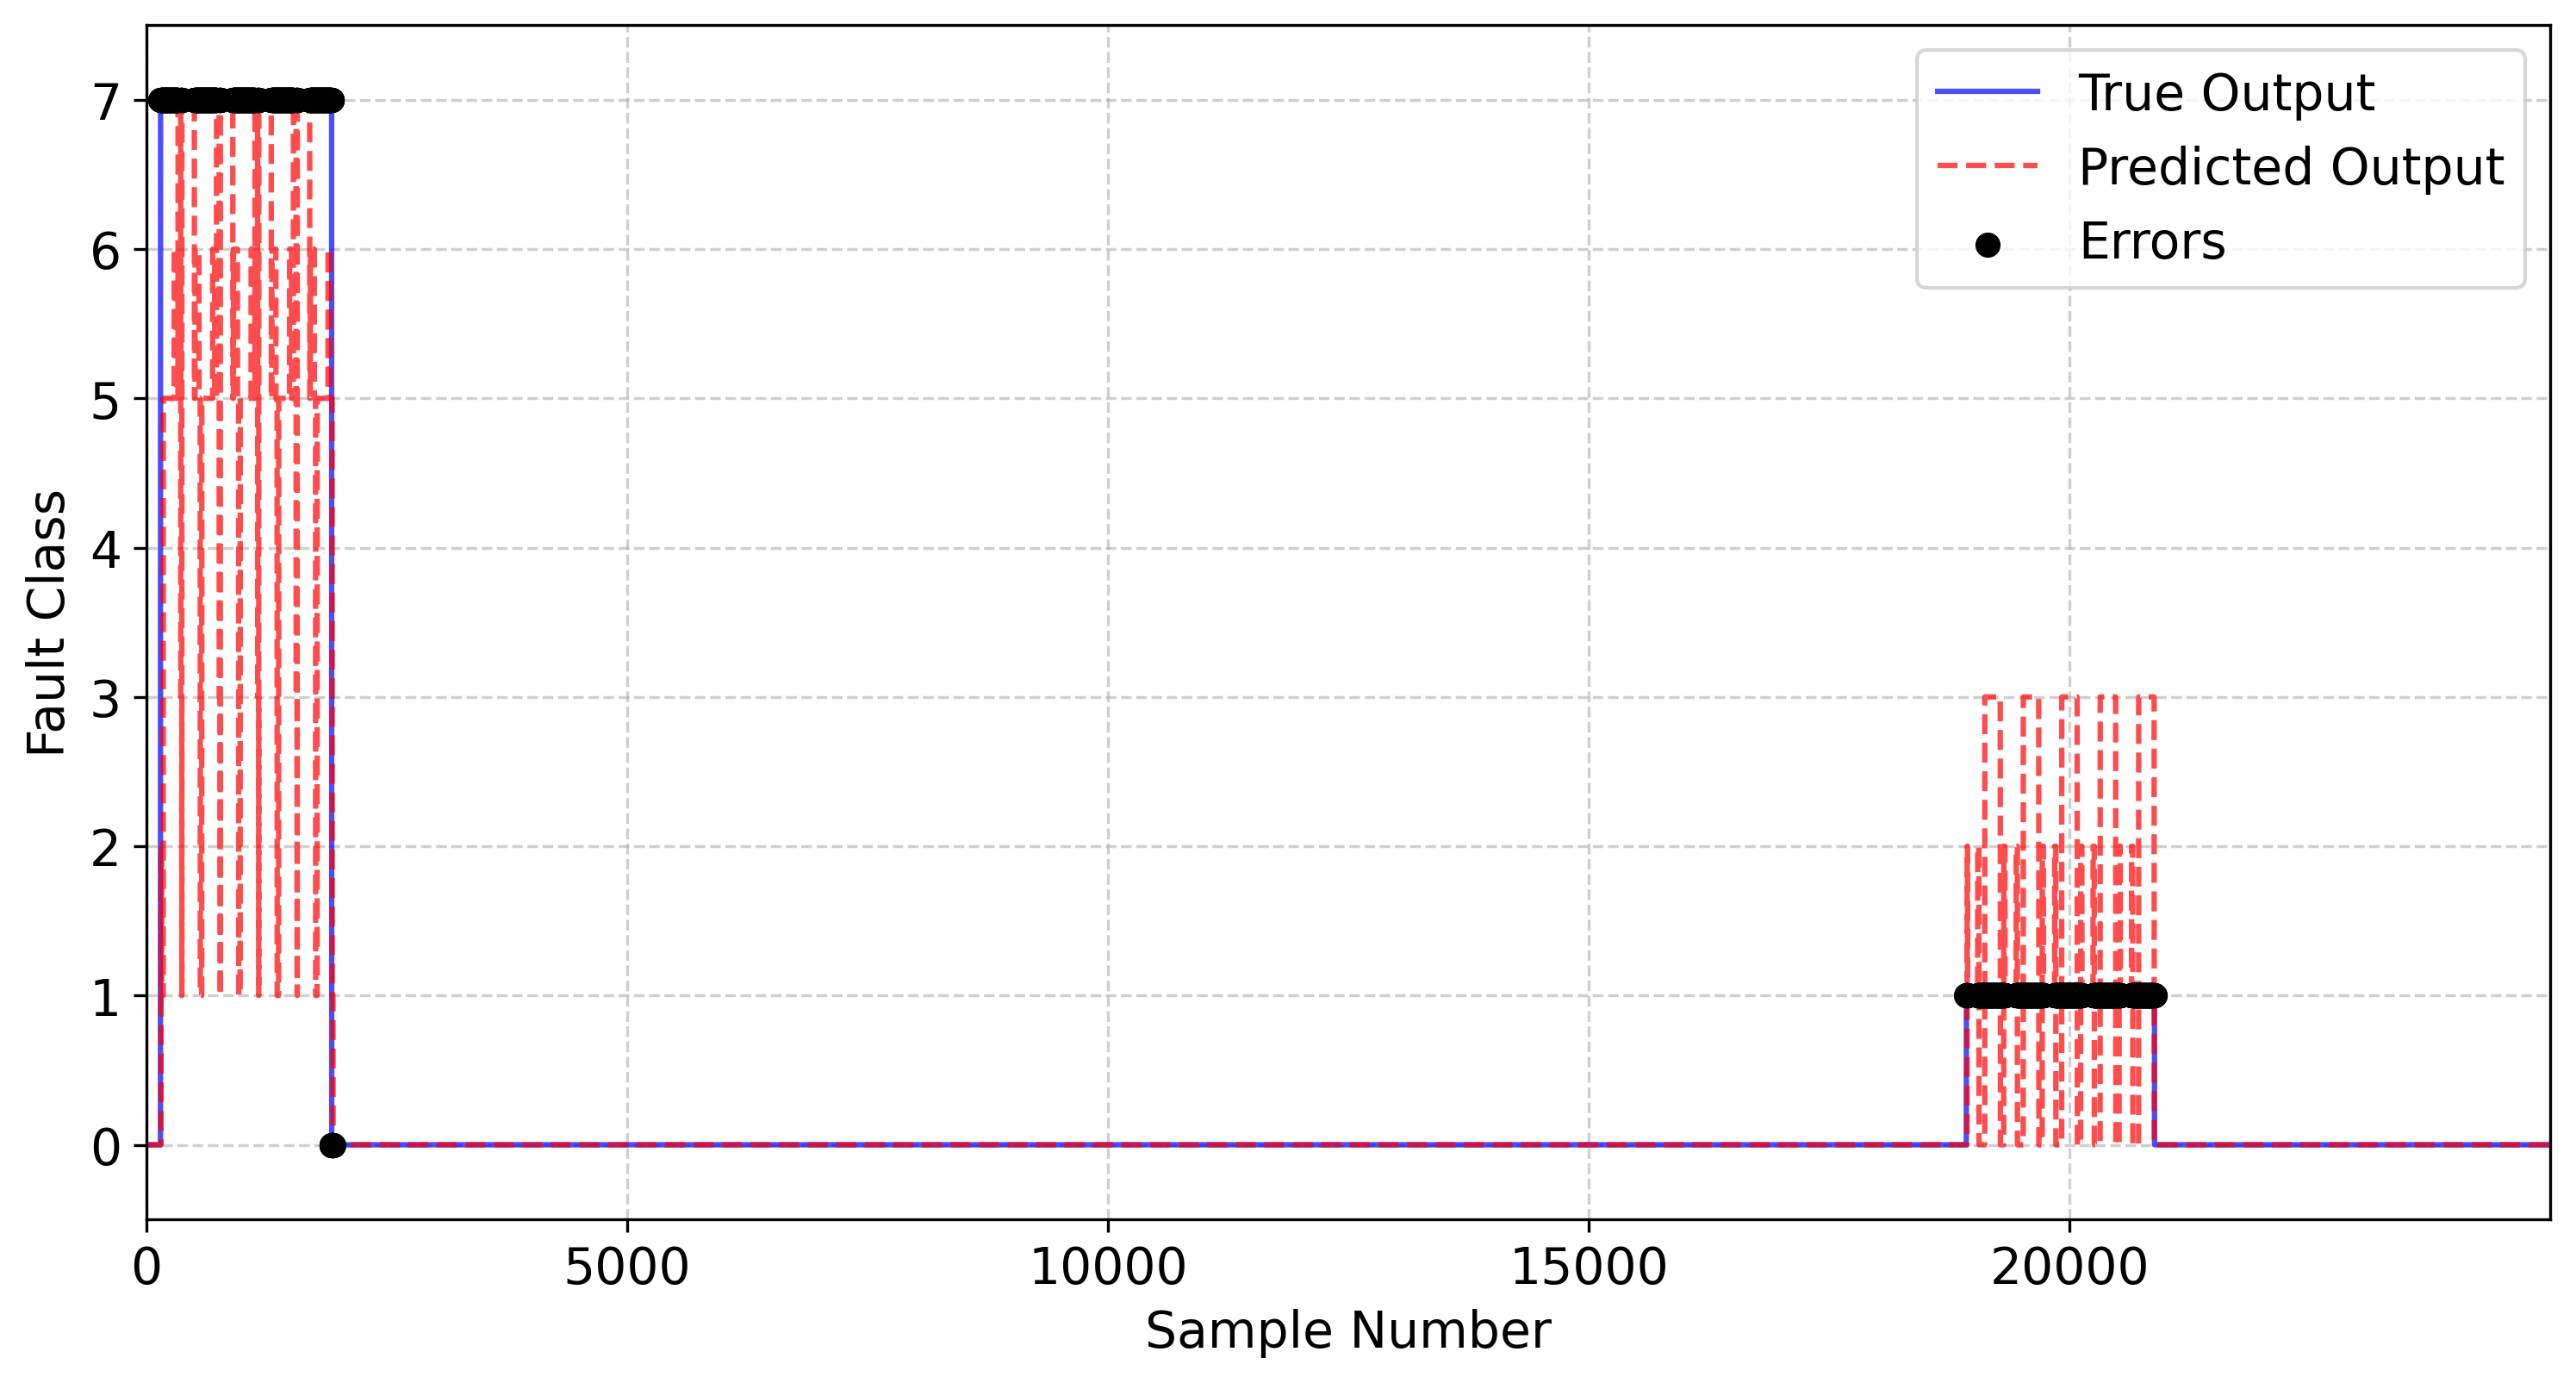
\includegraphics[width=1\linewidth]{figs/true_vs_predicted_gru_ekstra_minimum_model_window_size_15.png}
    \caption{GRU model with 2 neurons and a window size of 15}
    \label{fig:ekstra_minimum}
\end{figure}
Figure \ref{fig:4} presents the prediction of the GRU model with 16 neurons and a window size of 16. It is easy to notice that fault detection is much more stable and does not exhibit oscillations as in the previous two models.

\begin{figure}[H]
    \centering
    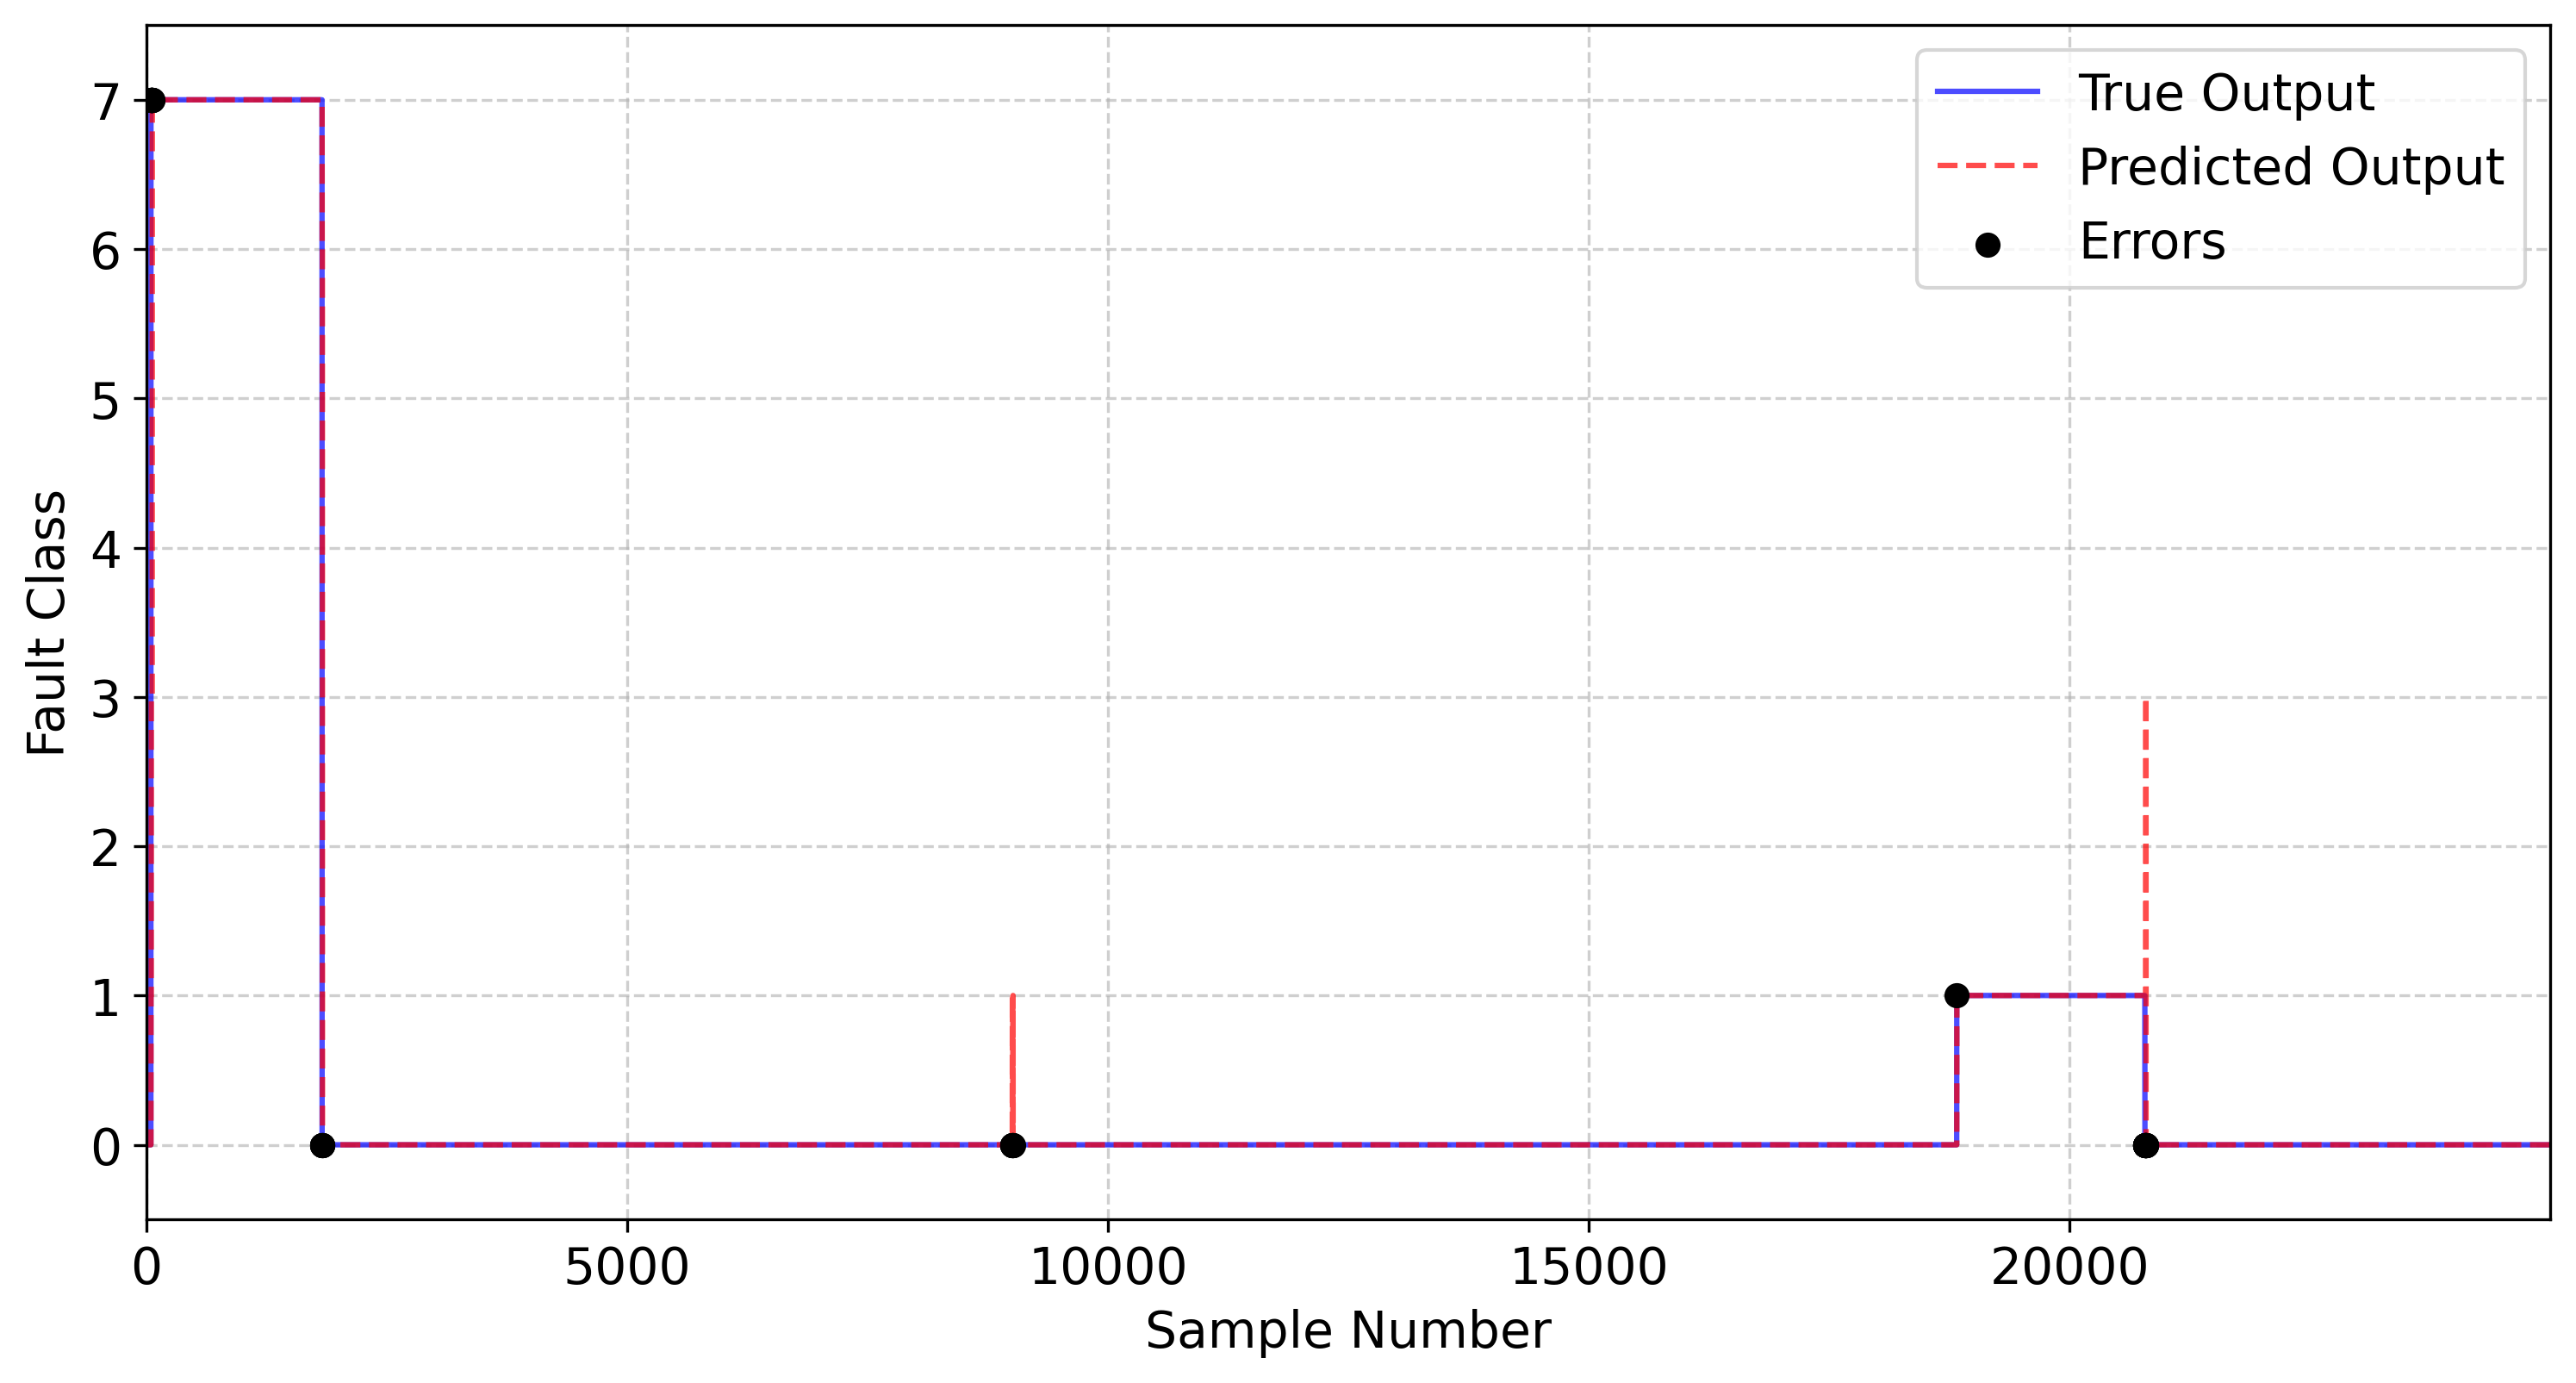
\includegraphics[width=1\linewidth]{figs/true_vs_predicted_gru_model_window_size_15.png}
    \caption{GRU model with 16 neurons and a window size of 15}
    \label{fig:4}
\end{figure}
Figure \ref{10} compares the actual and predicted outputs of the LSTM model for short circuit detection using a window size of 10. Important to note is that this model has two LSTM layers in the background working, so it is pretty computational complex. The model shows high accuracy, and good timing, no missed faults. But errors are noticeable during transitions between different faults, suggesting that the model may struggle with recognizing sudden changes accurately but for protecting the system the model is very reliable. This behavior is very similar to that of the GRU model with 18 neurons and a window size of 16. Despite this, the predictions are generally stable, and the model is capable of \textit{real-time} fault detection with a high degree of reliability.

\begin{figure}[H]
    \centering
    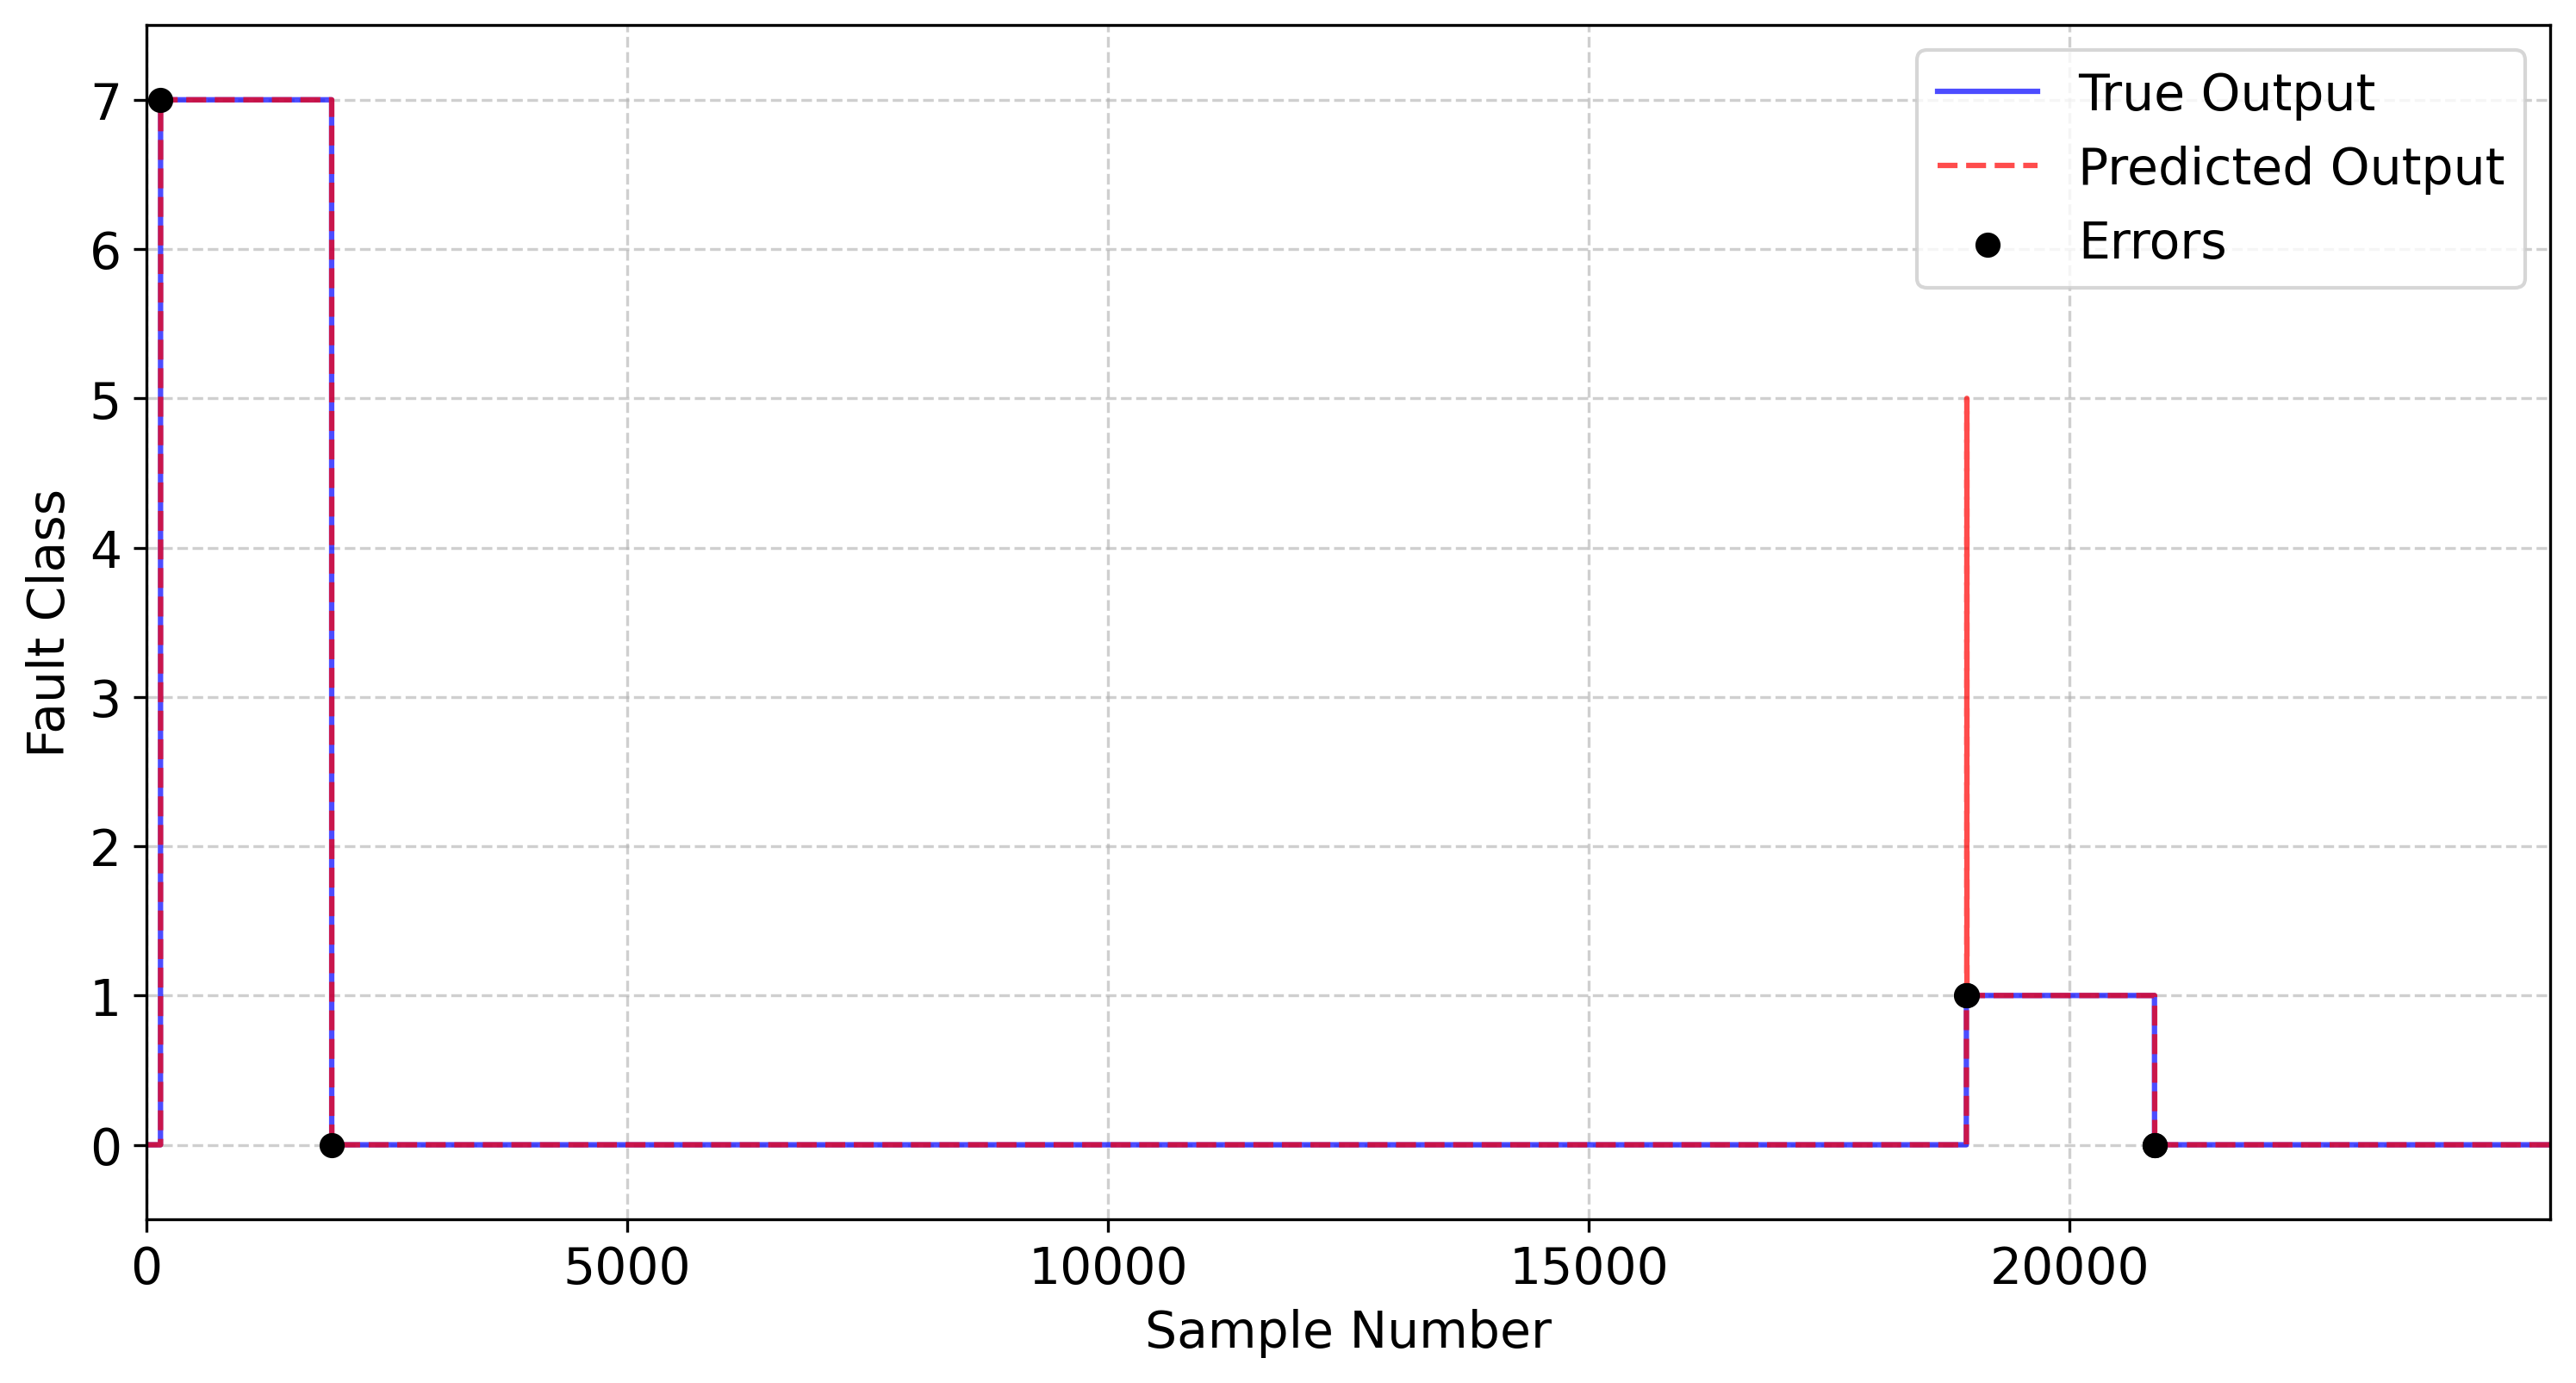
\includegraphics[width=\linewidth]{figs/true_vs_predicted_model_window_size_10.png}
    \caption{LSTM model with a window size of 10}
    \label{10}
\end{figure}

The graph \ref{fig:11} below presents a comparison of actual and predicted outputs of the LSTM model for short circuit detection using a window size of 15. In this case we are using only one LSTM layer but we are using more previous samples.

\begin{figure}[H]
    \centering
    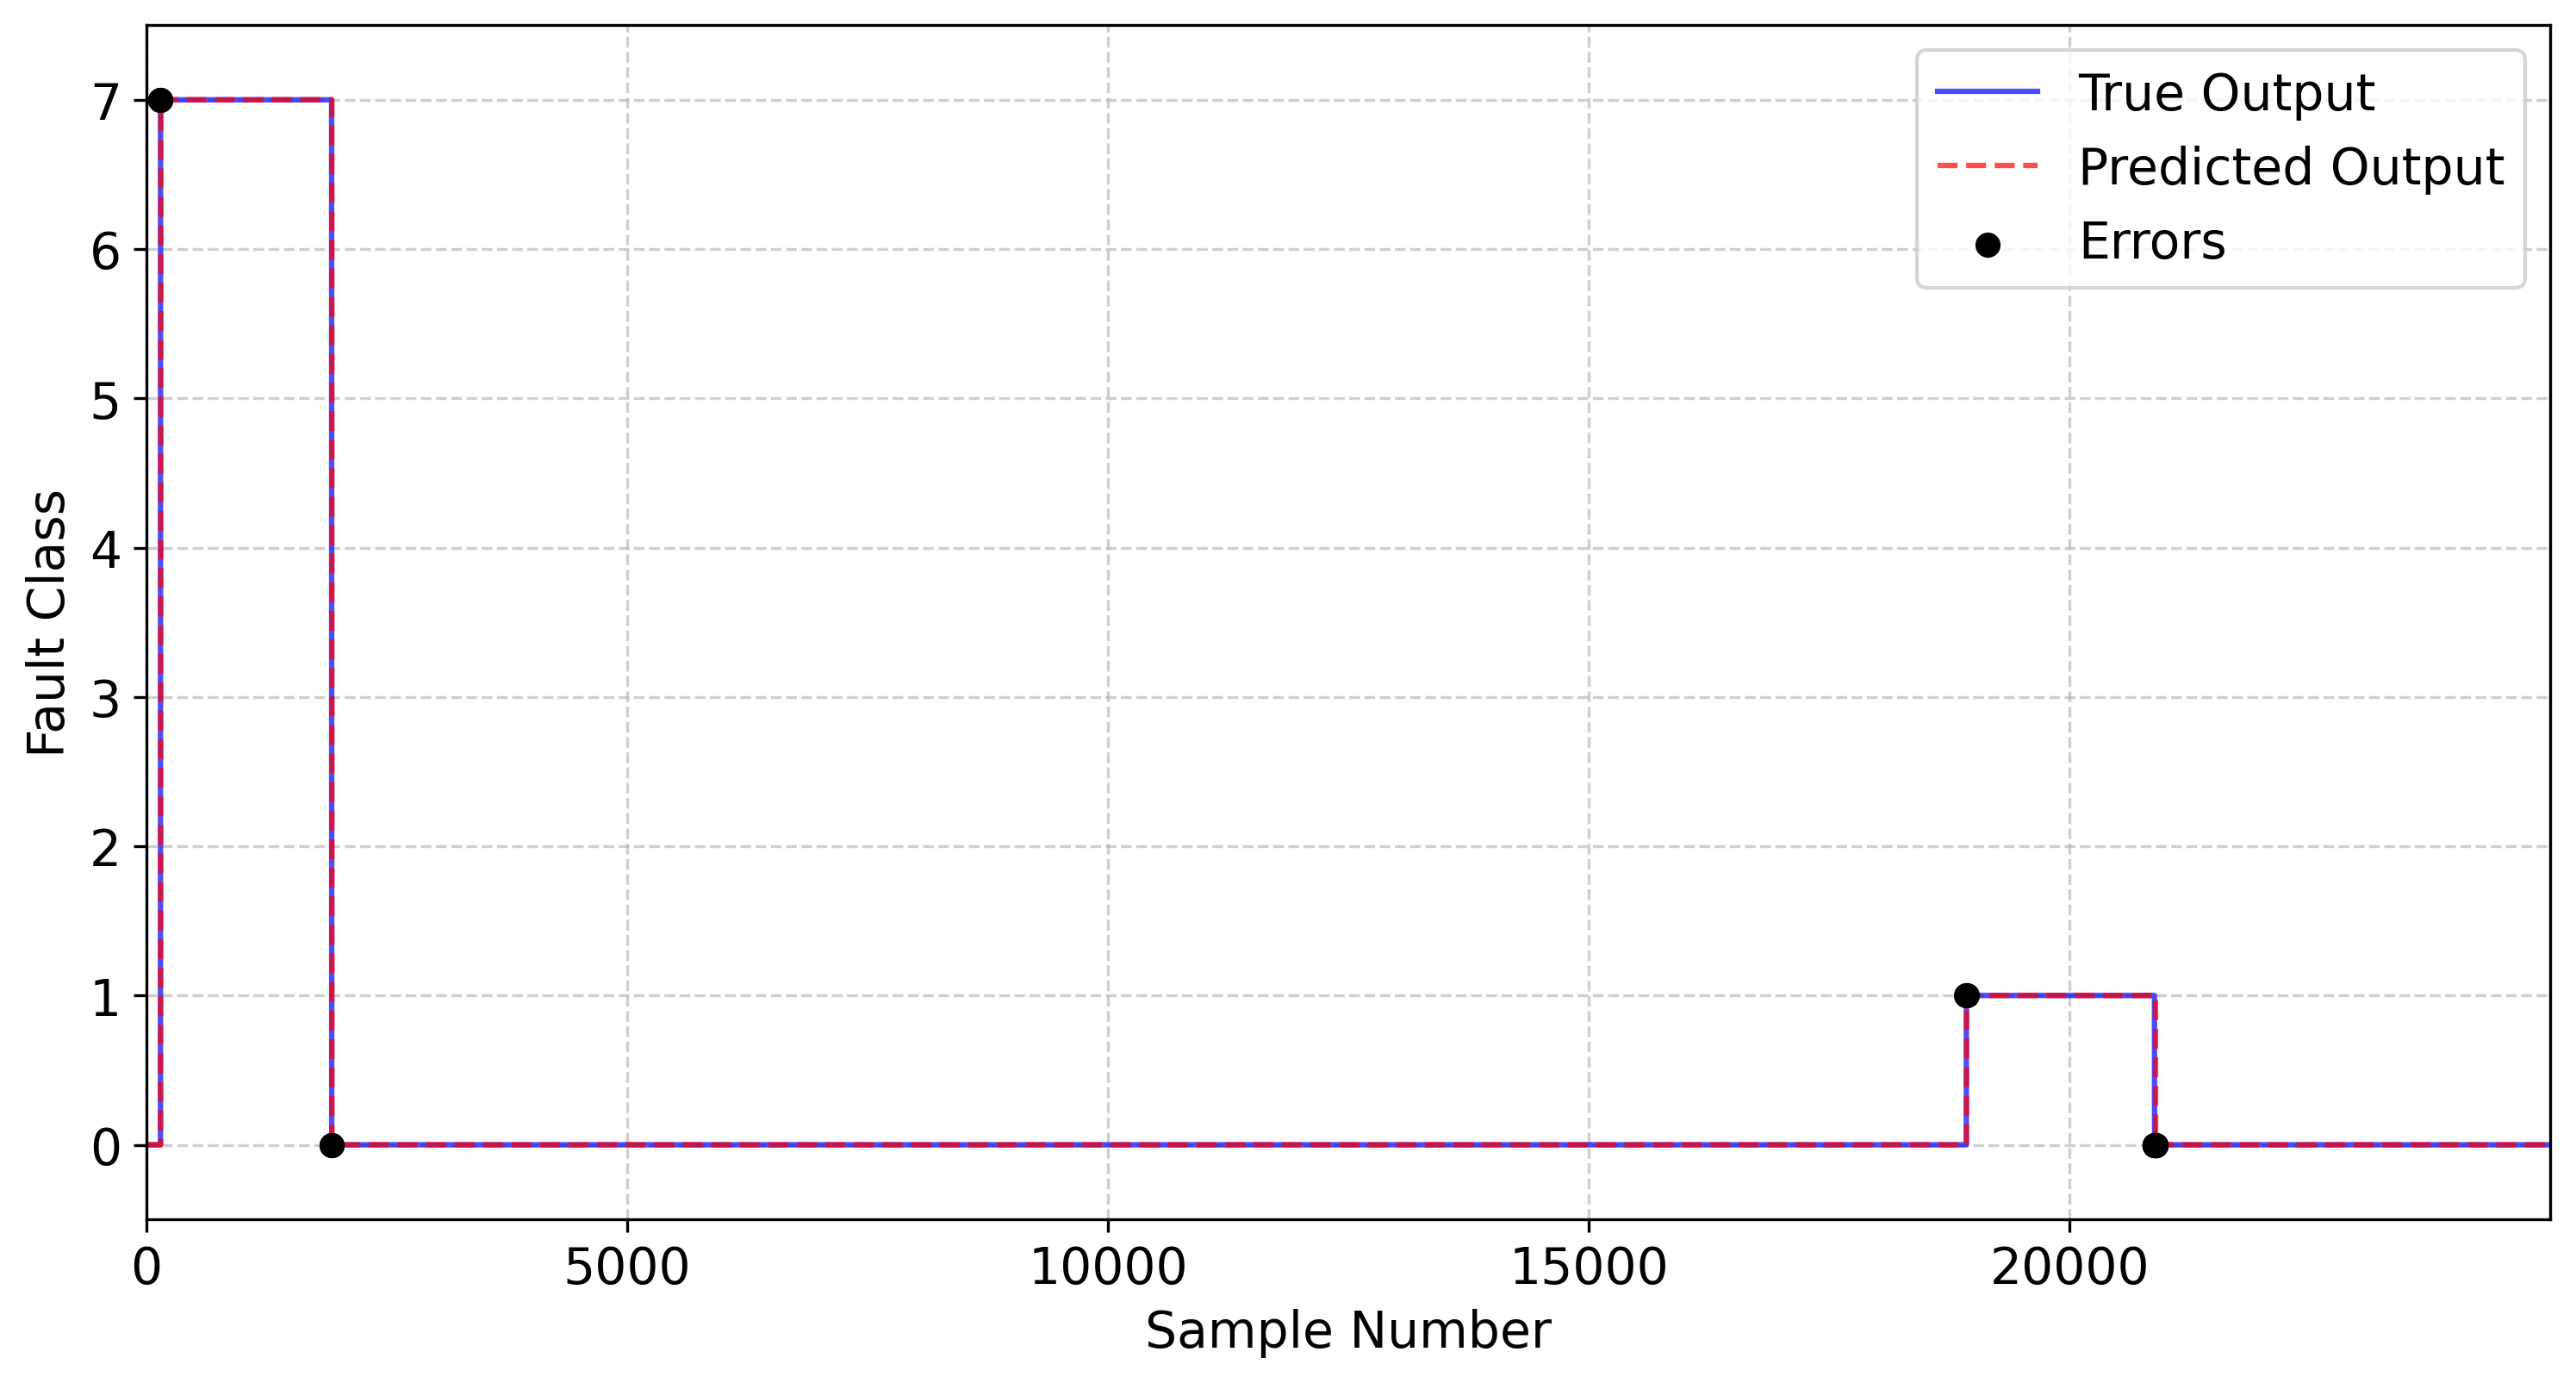
\includegraphics[width=1\linewidth]{figs/true_vs_predicted_model_window_size_15.png}
    \caption{LSTM model with a window size of 15}
    \label{fig:11}
\end{figure}
From Figure \ref{fig:11}, it is clear that this model shows the best accuracy in real-time fault detection. It is evident that the model does not exhibit undesirable fluctuations, making fault detection precise, timely, and reliable. The only drawback of this model is its computational complexity due to the large number of parameters. However, in today's era of extremely fast CPUs and GPUs with high levels of parallelism, this model is practically feasible. On figure \ref{fig:transition} we have shown the detection deley. On the figure it can be noted that the detection deley is small and is equal less than 20 samples. In practical terms if we would have a sampling rate of 20000 Hz the detection delay would be around 1 ms.
\begin{figure}[H]
    \centering
    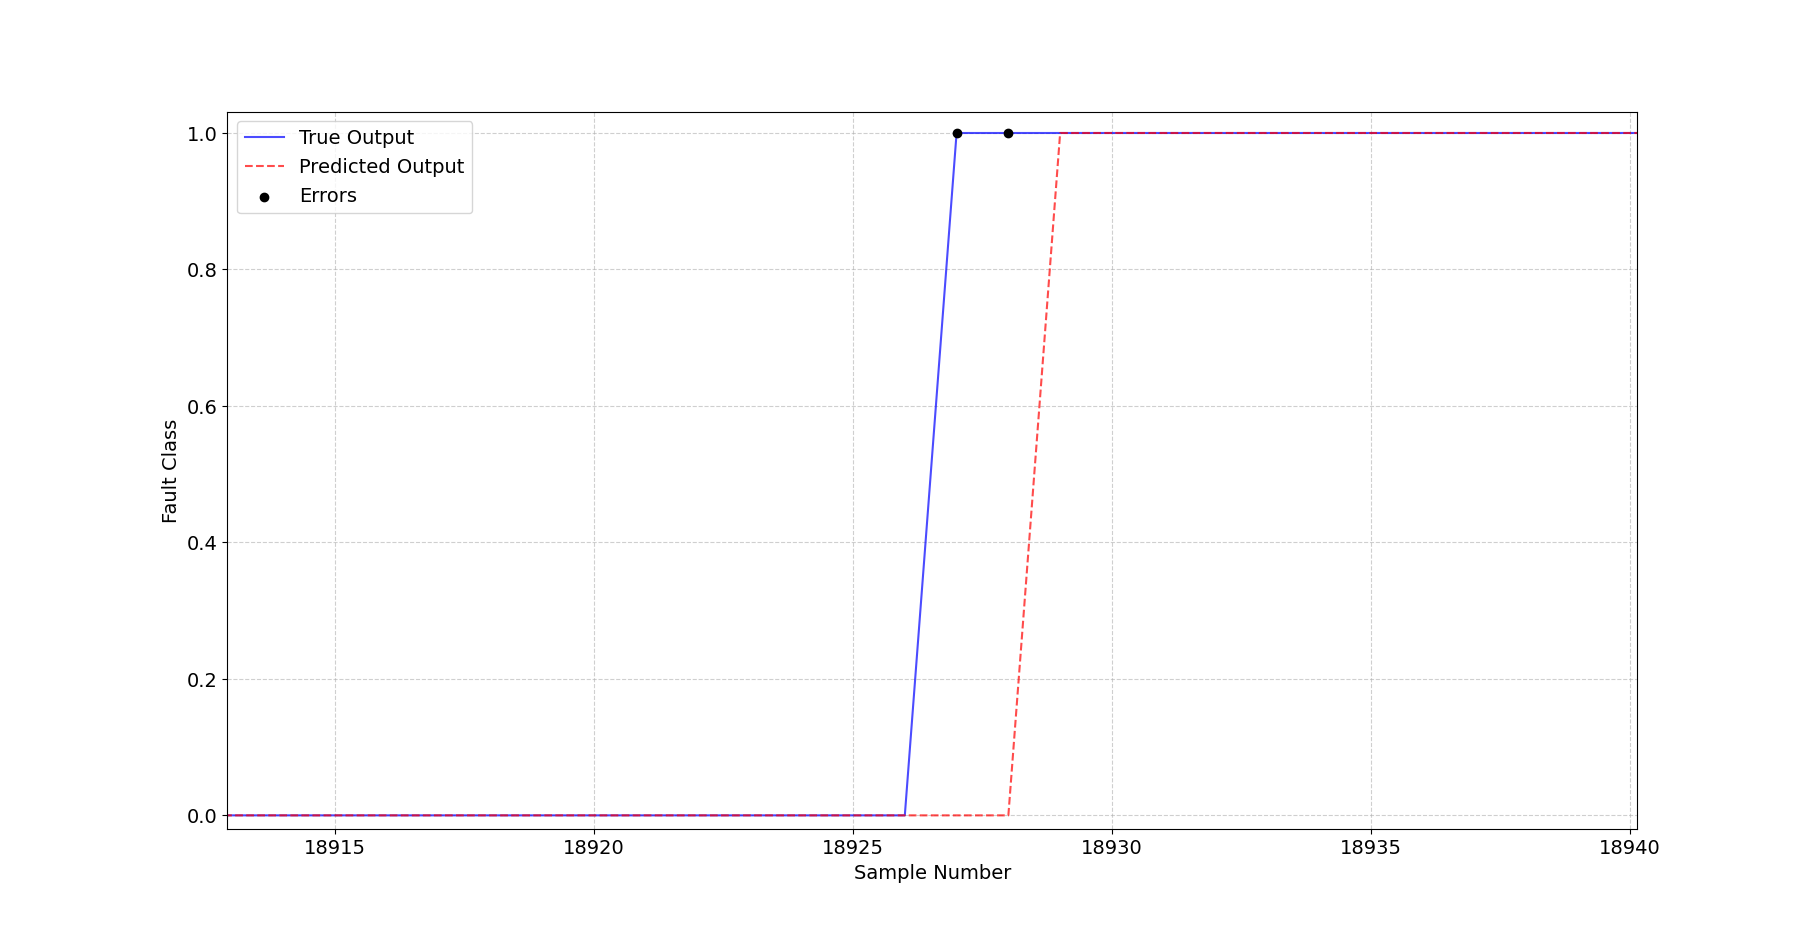
\includegraphics[width=\linewidth]{figs/transition.png}
    \caption{Moment of detection}
    \label{fig:transition}
\end{figure}

The simulation results indicate that GRU and LSTM neural networks can efficiently classify short circuits in real time, but the model's accuracy significantly depends on the time window size and the number of neurons (parameters). Models with longer time windows and a higher number of neurons generally show greater accuracy, while errors most commonly occur during fault transition states. Further optimization may involve improving regularization and fine-tuning hyperparameters to enhance model robustness. The detection delay is dependent on the sampling rate and the relation is inverse proportional with increase in the sampling rate we get a smaller detection delay.

\section{Conclusion}
This paper presents the implementation of deep learning for fault detection and classification in power system transmission lines. Using GRU and LSTM neural networks, an analysis was conducted on how different network architectures and training parameters affect fault classification accuracy.

The results show that a larger time window contributes to higher model accuracy, with LSTM achieving 99.85\% accuracy with a window size of 15, while GRU with 16 units achieves 99.16\% accuracy. Error analysis revealed that the network most frequently makes mistakes during sudden changes in the system, suggesting the need for further model optimization.

It is concluded that the application of neural networks in \textit{real-time} fault detection can significantly improve the security and stability of power systems. Future work may include hyperparameter optimization, improving model regularization, and testing on real-world data from power networks.

NOTE: The implemented code is available on the GitHub repository, accessible by clicking on \textit{https://github.com/Spago123}.

\bibliographystyle{ieeetr}
\bibliography{Bibliography}

\end{document}
